\documentclass[12pt,a4paper]{article}% 

\usepackage[a4paper,margin=1in]{geometry}
\usepackage{kbordermatrix}
\usepackage{amsmath}
\usepackage{pgfplots}
\usepackage{mathtools}
\usepackage{blindtext}
\usepackage{graphicx}
\usepackage{enumitem}
\usepackage{xcolor}
\usepackage{tikz}
\usepackage{algorithm}
\usepackage{textcomp}
\usepackage[noend]{algorithmic}
\usepackage{listings}
\DeclarePairedDelimiter{\ceil}{\lceil}{\rceil}
\DeclarePairedDelimiter\floor{\lfloor}{\rfloor}
\lstset{
	frame=tb, % draw a frame at the top and bottom of the code block
	tabsize=4, % tab space width
	showstringspaces=false, % don't mark spaces in strings
	numbers=left, % display line numbers on the left
	commentstyle=\color{green}, % comment color
	keywordstyle=\color{blue}, % keyword color
	stringstyle=\color{red} % string color
}

\usepackage [english]{babel}
\usepackage [autostyle, english = american]{csquotes}
\MakeOuterQuote{"}
\usepackage{pgfplots,amsmath}
\pgfplotsset{compat=1.12}



\newcommand{\TITLE}[1]{\item[#1]}
\renewcommand{\algorithmiccomment}[1]{$/\!/$ \parbox[t]{4.5cm}{\raggedright #1}}
\newbox\fixbox
\renewcommand{\algorithmicdo}{\setbox\fixbox\hbox{\ {} }\hskip-\wd\fixbox}
\newcommand{\algcost}[2]{\strut\hfill\makebox[1.5cm][l]{#1}\makebox[4cm][l]{#2}}
\usetikzlibrary{arrows,automata,positioning}
\usetikzlibrary{arrows.meta}
\usetikzlibrary{calc}

\pgfmathsetseed{3}
\newcommand*{\Comb}[2]{{}^{#1}C_{#2}}

\begin{document}
	
	
	\begin{titlepage}
		\title{
\includegraphics[width=0.38 \textwidth]{./NIT_Silchar_logo.png}\\\textbf{\large NATIONAL INSTITUTE OF TECHNOLOGY, SILCHAR}\\\textbf{{\large Department of Computer Science and Engineering}}\\\bigskip {\large Project Report on,}\\\bigskip\textbf{{\normalsize ALGORITHMS }}}
		\author{Subject : Algorithms (CS-$206$)\\\\ Submitted by,\\Name : Arvinder Singh\\Scholar ID : 18-1-5-126\\B.Tech 4th SEM (CSE)}
		\date{\today}
		\clearpage\maketitle
		\thispagestyle{empty}
	\end{titlepage}
	
	\begin{center}
		\textbf{\large ABSTRACT}
	\end{center}
    \begin{flushleft}  \fontsize{12pt}{18pt}\selectfont
		"In this project report, I have tried to give a concise overview on my approach to solve the given problem statement in the most optimal and feasible way.\\\bigskip Starting with the project description I have tried to devise my approach in tackling the problem. Then gradually I have build up the algorithm. Later I have proved the correctness of my designed algorithm using mathematical induction. Later I have justified the paradigm used in my solution. \\\bigskip Rigorous time complexity analysis is done at the end. Example input and output for the algorithm is also shown alongwith step-wise running of the algorithm and final output is obtained. Lastly, some drawbacks of the algorithm is also discussed.\\\bigskip This project is developed using one of the open source software \LaTeX\\." 
	\end{flushleft}
	
	\pagebreak
	\tableofcontents
	\cleardoublepage
	\section{Project Description}\label{sec:intro}
	\begin{flushleft}
		In this project we develop an algorithm that converts the given input which is in \textit{integer (base $10$)} format to \textit{binary (base $2$)} representation. We use one of the algorithm paradigms \textit{Divide and Conquer} to achieve this. We exploit given procedure \textsc{Fast-Multiply}$(x,y)$ to achieve this for performance reasons \textit{(discussed later)}.\\\bigskip
		We devise two algorithms \textsc{Bin-Pow-Ten}$(n)$ which takes a single parameter $n$ and raises $10$ to the power $n$ and returns the value in binary. Also, another function \textsc{Dec-To-Bin}$(x)$ is devised to convert \textit{decimal} or \textit{integer} value to \textit{binary}.\\\bigskip
		In the following section we will give the concise algorithm for all the procedures.
	\end{flushleft}
	\section{Algorithm}
	In this section I have given algorithms for the functions described in above, \textit{i.e.,} \textsc{Fast-Multiply}$(x,y)$, \textsc{Bin-Pow-Ten}$(n)$ and \textsc{Dec-To-Bin}$(x)$. For simplifying our analysis we consider cost of all operations to be $1$. The addition and multiplications of $2$ takes linear time since it is merely \textit{left shifts}. \bigbreak
	\begin{itemize}
	\item{
		\begin{algorithmic}[1]
		\TITLE{\textsc{Fast-Multiply}$(x,y)$}\COMMENT{$x,y \rightarrow$ \textit{binary numbers} }\\
		\textbf{Input}: $x=1011_2, y=1110_2$\\
		\textbf{Output}: $1001010_2$
		\algcost{\textit{Cost}}{}
		\STATE $\mathit{n} = max$(no. of bits of $x$, no. of bit of $y)$
		\algcost{$\mathcal{O}(1)$}{}
		\IF{$ \mathit{n}=1 $}
		\STATE{$\mathit{return}\enspace xy$}
		\algcost{$\mathcal{O}(1)$}{}
		\ENDIF
		\STATE $x_L,x_R=leftmost\ceil{\frac{n}{2}},rightmost\floor{\frac{n}{2}}\enspace of\enspace x$ 
		\algcost{$\mathcal{O}(1)$}{}
		\STATE $y_L,y_R=leftmost\ceil{\frac{n}{2}},rightmost\floor{\frac{n}{2}}\enspace of\enspace y$
		\algcost{$\mathcal{O}(1)$}{}
		\STATE $M_1 =$ \textsc{Fast-Multiply}$(x_L,x_R)$
		\algcost{$T(\frac{n}{2})$}{}
		\STATE $M_2 =$ \textsc{Fast-Multiply}$(y_L,y_R)$
		\algcost{$T(\frac{n}{2})$}{}
		\STATE $M_3 =$ \textsc{Fast-Multiply}$(x_L+x_R,y_L+y_R)$
		\algcost{$T(\frac{n}{2})$}{}
		\STATE{$\mathit{return}\enspace 2^{n} M_1 + 2^{\frac{n}{2}} (M_3 - M_1 - M_2 ) + M_2 $}
		\algcost{$\mathcal{O}(n)$}{}
		\end{algorithmic}
	}\bigskip
	\item{
		\begin{algorithmic}[1]
			\TITLE{\textsc{Bin-Pow-Ten}$(n)$}\COMMENT{$n \rightarrow$ \textit{power to which 10 is to be raised} }\\
			\textbf{Input}: $n=2$\\
			\textbf{Output}: $1100100_2$
			\algcost{\textit{Cost}}{}
			\IF{$ \mathit{n}=1 $}
			\STATE{$\mathit{return}\enspace 1010_2$}
			\algcost{$\mathcal{O}(1)$}{}
			
			\ELSE
			\STATE {$a=$\textsc{Bin-Pow-Ten}$(\frac{n}{2})$}
			\algcost{$G(\frac{n}{2})$}{}
			\STATE {$return \enspace$\textsc{Fast-Multiply}$(a,a)$}
			\algcost{$\mathcal{O}(n^{log_2 {3}})$}{}
			\ENDIF
		\end{algorithmic}
	}\bigskip\break
	\item{
			\begin{algorithmic}[1]
			\TITLE{\textsc{Dec-To-Bin}$(x)$}\COMMENT{$x \rightarrow$ \textit{number which need to be converted to binary} }\\
			\textbf{Input}: $x=13$\\
			\textbf{Output}: $1101_2$
			\algcost{\textit{Cost}}{}
			\STATE{initialize bin[0...9] with all the binary values\\ n $\leftarrow$ is the number of digits in $x$}
			\algcost{$\mathcal{O}(1)$}{}
			\IF{$ \mathit{n}=1 $}
			\STATE{$\mathit{return}\enspace bin[x]$}
			\algcost{$\mathcal{O}(1)$}{}
			\ELSE
			\STATE $x_L,x_R=leftmost\frac{n}{2},rightmost\frac{n}{2}\enspace of\enspace x$ 
			\algcost{$\mathcal{O}(1)$}{}
			\STATE{$\mathit{return}$  \textsc{Fast-Multiply}$(\textsc{Bin-Pow-Ten}$($\frac{n}{2}$)$,\textsc{Dec-To-Bin}(x_L))$\\$+\textsc{Dec-To-Bin}(x_R)$}
			\algcost{$2H(\frac{n}{2})+G(\frac{n}{2})+T(\frac{n}{2})$}{}
			\ENDIF
		\end{algorithmic}
	}
	\end{itemize}



	\section{Proof of Correctness}
	\begin{flushleft}
		First of all we will prove the correctness of the \textsc{Fast-Multiply}$(x,y)$ algorithm, using structural induction of this recursive algorithm itself.\\\smallskip
		In this algorithm we know that the inputs is power of $2$ as given in the problem statement. Also, in induction we first prove the \textit{Basis} step and then move on to proving the \textit{inductive} step. We also have to prove that the the algorithm terminates and that if it terminates then, the preconditions imply the postconditions. \\\smallskip
		We know that the algorithm terminates because the number of bits in each successive recursive call is strictly decreasing sequence belonging to the natural numbers,\textit{i.e.,} $\in \mathbf{N} $.
		\\\smallskip
		\textbf{Proof}:
		\\\smallskip
		Let the statement be $T(n)$ : Number of bits in the input.\\\bigskip
		\textit{Basis}: If the length of the input numbers is $1$. The algorithm simply multiply the two numbers and return it. Hence, the basis step is proved.\\\bigskip
		\textit{Inductive}: Let us assume that the algorithm is correct for $T(k)$ we have to prove that the algorithm is correct for $T(k')$, where $k'>k$, in fact for our input $k'$ is nothing but $k'=2k$. We do this by showing that the combined step is indeed correct.\\\smallskip
		We know that multiplication of any two binary numbers is $xy=(2^{k/2} x_L +x_R)(2^{k/2} y_L +y_R)$, where $k$ is the length of the maximum of the length of the two numbers $x$ and $y$. Also, the above can be simplified to shown to be,
		$2^{k} x_L y_L + 2^{\frac{k}{2}} ((x_L +x_R)(y_L +y_R) - x_L x_R - y_L y_R ) + x_R y_R $.\\\smallskip
		The above combined step is indeed correct which is actually what is in the algorithm. This proves our inductive step. Therefore, this algorithm holds for $k'$.\\\smallskip
		Therefore, by the principle of mathematical induction we proved the correctness of our first algorithm.\\\bigskip
		
		We now prove the working the second algorithm,\textit{i.e.,} \textsc{Bin-Pow-Ten}$(n)$ it is almost exactly same as the above except in the \textit{basis} step it returns the actual value of $10$ in \textit{binary}. Also, the combined step in the inductive process we have the \textsc{Fast-Multiply}$(x,y)$ algorithm which is already proved. \\\smallskip 
		So, all the requirements of the proof is satisfied and hence this second algorithm is also proved to be correct.\\\bigskip
		
		We now move to our final algorithm which combines the functionalities of the above two algorithms to solve our problem in the problem statement. This is the \textsc{Dec-To-Bin}$(x)$ algorithm. It has also the same structural proof as in the first algorithm. In the \textit{basis} step \textit{i.e.,} at $n=1$ it simply  return the actual binary value of the decimal number stored in the memory, so the basis step is proved to be correct. In the inductive step again we just use our helper algorithms which are already proved to be correct tp return the result.\\\smallskip
		So, this completes our proof and this section as well.
		
	\end{flushleft}

	
	
	
	
	
	\section{Justification of Solution}
	\begin{flushleft}
	To convert decimal integer to binary we have used the divide and conquer paradigm. The reason behind using this technique is that the problem get divided into smaller problems and we find solutions to those smaller problems, combine them in next step and build our solution ground up.\\\smallskip
	In our initial approach of this divide and conquer algorithm for binary number multiplication we have the multiplication of the two numbers as follows:\\\smallskip
	\begin{center}
		$xy=(2^{\frac{n}{2}} x_L + x_R)(2^{\frac{n}{2}} y_L+y_R)$\\
	\end{center}
	where $x_L,x_R$ are the two equal parts of $x$ of length $\frac{n}{2}$ namely left half and right half, similarly for $y$. $n$ is the number of bits in maximum of $x$ or $y$.

	\begin{equation}
		\implies xy = 2^{n} x_L y_L + 2^{\frac{n}{2}} ( x_L y_R + x_R y_L ) + x_R y_R 
	\end{equation}
	The recurrence relation for the above equation if we write an algorithm for it is $T(n)=4T(\frac{n}{2})+\mathcal{O}(n)$.
	\\\smallskip
	The time-complexity upon solving the above equation (\textit{discussed in the complexity section}) is $\approx \mathcal{O}(n^{2})$. This is the time-complexity of the un-optimized algorithm, we can do even better than that.\\\smallskip 
	In the eq.($1$) we see that there is multiplication of $4$ terms. There, exists a very clever observation which allows us to do the same multiplication of $x$ and $y$ in $3$ operations. This is the new optimized approach. Upon observation we see that the term $( x_L y_R + x_R y_L )$ in equation ($1$) can be written as,
	$((x_L +x_R)(y_L +y_R) - x_L y_L - x_R y_R )$. This greatly reduced the number of multiplications made, only a few addition operations are introduced which takes lesser time as compared to another multiplication. Upon writing the recurrence relation for this algorithm we have the recurrence relation as $T(n)=3T(\frac{n}{2})+\mathcal{O}(n)$. Just the factor $4$ in previous recurrence changes to $3$. If we solve this relation then we have the time-complexity as $\mathcal{O}(n^{log_2 {3}}) \approx \mathcal{O}(n^{1.59})$.\\\smallskip
	From the above discussion we can see that this is a huge improvement from the previous approach. Just a small tweak had so large a impact on the complexity of the algorithm.
	\end{flushleft}
	\break

	\section{Time Complexity Analysis}
	\begin{flushleft}
		Before we begin the analysis of the algorithm we will be using master's theorem for finding the time complexities of the recurrence relation, which is stated as follows:\\\smallskip
		If $T(n)=aT(\ceil{\frac{n}{b}})+\mathcal{O}(n^d)$ for some constants $a > 0, b>1,$ and $d \geq 0$,then\\
		\begin{equation}
		%	\[
			T(n)= 
			\begin{cases}
			\mathcal{O}(n^d),& if d>log_b {a}\\
			\mathcal{O}(n^d log {n}) ,& if d=log_b {a}\\				\mathcal{O}(n^{log_b {a}}) ,& if d<log_b {a}\\
			\end{cases}
		%	\]
		\end{equation}
		
	\end{flushleft}
	
	\begin{itemize}
		\item{
			\begin{flushleft}
				We first analyze the time complexity of our first algorithm \textsc{Fast-Multiply}$(x,y)$. Let the cost of this algorithm is $T(n)$. In the \textit{section} $2$ we have already shown the cost of each step of this algorithm now we write the recurrence relation for it,which is as follows:\\
				\begin{equation}
					T(n) = 3T(\frac{n}{2}) + \mathcal{O}(n)
				\end{equation}
				if we compare the above equation with that in equation ($2$), we have $d=1$ and $log_2 {3}$ and $d<log_2 {3}$ so, from the third case of the master's theorem we have,\\
				\begin{center}
					$T(n)=\mathcal{O}(n^{log_2 {3}})\approx \mathcal{O}(n^{1.59})$
				\end{center}
				Next we move on to our second algorithm.
			\end{flushleft}
		}
	  \item{
	  	\begin{flushleft}
	  		We first analyze the time complexity of our second algorithm \textsc{Bin-Pow-Ten}$(n)$. Let the cost of this algorithm is $G(n)$. In the \textit{section} $2$ we have already shown the cost of each step of this algorithm now we write the recurrence relation for it,which is as follows:\\
	  		\begin{equation}
	  		G(n) = G(\frac{n}{2}) + \mathcal{O}(n^{log_2 {3}})
	  		\end{equation}
	  		if we compare the above equation with that in equation ($2$), we have $d=log_2 {3}$ and $log_2 {1}=0$ and $d>0$ so, from the first case of the master's theorem we have,\\
	  		\begin{center}
	  			$G(n)=\mathcal{O}(n^{log_2 {3}})\approx \mathcal{O}(n^{1.59})$
	  		\end{center}
	  		Upon observation we can see that the complexity is exactly same as the first algorithm. Next we move on to our final and the algorithm that solves the problem given in our problem statement.
	  		\end{flushleft}
	  	}
  	  \item{
  	  	\begin{flushleft}
  	  		We first analyze the time complexity of our last algorithm \textsc{Dec-To-Bin}$(x)$. Let the cost of this algorithm is $H(n)$. In the \textit{section} $2$ we have already shown the cost of each step of this algorithm now we write the recurrence relation for it,which is as follows:\\
  	  		\begin{equation}
  	  		H(n) = 2H(\frac{n}{2}) + G(\frac{n}{2}) + T(\frac{n}{2})
  	  		\end{equation}
  	  		
  	  		\begin{center}
  	  			$\implies H(n) = 2H(\frac{n}{2}) + \mathcal{O}({(\frac{n}{2})}^{log_2 {3}}) + \mathcal{O}({(\frac{n}{2})}^{log_2 {3}})$
  	  		\end{center}
    		The above equation simplifies to the following,
  	  		\begin{center}
  	  			$\implies H(n) = 2H(\frac{n}{2}) + \mathcal{O}({n}^{log_2 {3}})$
  	  		\end{center}
  	  		
  	  		if we compare the above equation with that in equation ($2$), we have $d=log_2 {3}$ and $log_2 {2}=1$ and $d>1$ so, from the first case of the master's theorem we have,\\
  	  		\begin{center}
  	  			$G(n)=\mathcal{O}(n^{log_2 {3}})\approx \mathcal{O}(n^{1.59})$
  	  		\end{center}
  	  		Upon observation we can see that the complexity is exactly same as the first two algorithm. Therefore the required complexity of our final algorithm is:\\
  	  		\begin{center}
  	  			$\boxed{\approx \mathcal{O}(n^{1.59})}$
  	  		\end{center}
    		This concludes our analysis for this section.
  	  	\end{flushleft}
  	  }
	\end{itemize}

	\section{Results and Discussion}
	\begin{flushleft}
		In this section we demonstrate the running of \textsc{Dec-To-Bin}$(x)$ algorithm. Each call to the respective function is shown as the following.\\
		
		For demonstrating the running of  our algorithm we take the following input: $2421_{10}$ and we will convert it to binary. The recursion tree for the example is shown as follows\\\bigskip
		\hspace*{-0.7in}
		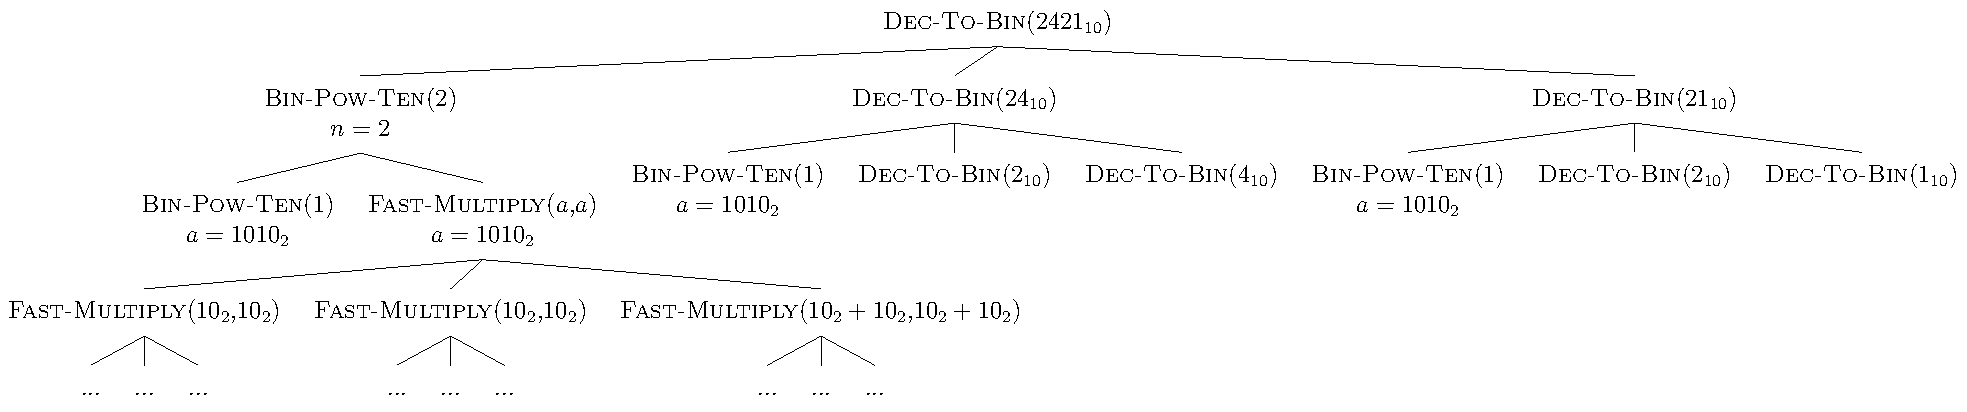
\includegraphics[scale=0.58]{./tree.pdf}
		From the above tree we can clearly see each successive step of the algorithm. The answer is generated from the bottom most calls first, then in their just next combination state the answer to another sub-problem is created, in this fashion the entire tree in the top-most node generates answer to our original problem. \\\bigskip
	%	\hspace*{-0.7in}
		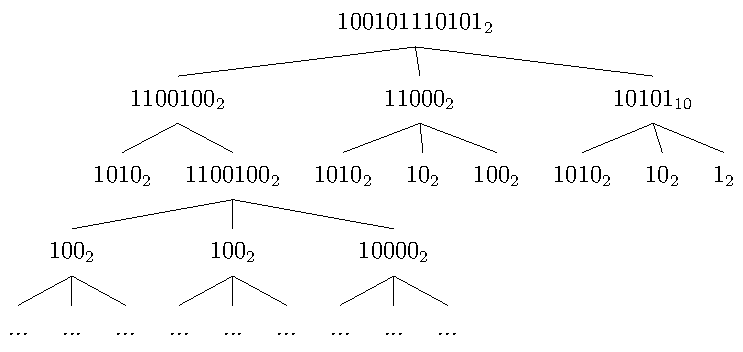
\includegraphics[scale=1]{./answertree.pdf}\\\bigskip
		The answer tree for the the first recursion tree is shown in the above diagram. The answers are combined by the formulas given in the algorithm itself.\\\smallskip
		Had this algorithm not been optimized as given by eq. ($1$) we would have had a recursion tree with at-most $4$ children, this would have affected the efficiency of the algorithm as we have already seen mathematically in the the complexity analysis section.
	\end{flushleft}
	\section{Drawbacks}
	\begin{flushleft}
		We have developed this algorithm only for decimal number conversion (\textit{i.e., base 10}), but this algorithm will not work for octal or hexadecimal numbers, there is room for improvement. As any input like \textsc{Dec-To-Bin}$(7_8)$ will give incorrect output. Otherwise for any decimal inputs the algorithm is flawless.
	\end{flushleft}
	
\end{document}